\documentclass[a4paper]{article}
\usepackage[left=2.1cm, right=2.1cm, top=2.1cm]{geometry}
\usepackage{lipsum}
\usepackage{tikzpagenodes}
\usepackage{pgfplots}
\usepackage{tikz}
\usepackage{tikz-3dplot}
\usetikzlibrary{arrows,decorations.pathmorphing,backgrounds,positioning,fit,matrix}
\pgfplotsset{compat=1.8}
\usepackage{graphics} % for pdf, bitmapped graphics files
\usepackage{epsfig} % for postscript graphics files
\usepackage[colorlinks=true,citecolor=green]{hyperref}
\usepackage{cite}
\usepackage{amsmath,amssymb,amsfonts}
\usepackage{algorithmic}
\usepackage{graphicx}
\usepackage{url}
\usepackage{cite}
\usepackage{bm}
\usepackage{pbox}
\usepackage{siunitx,booktabs,etoolbox}
\usepackage{ulem}
\usepackage[framed,numbered,autolinebreaks,useliterate]{mcode}
\usepackage{filecontents}
%\usepackage{bigfoot} % to allow verbatim in footnote


\def\BibTeX{{\rm B\kern-.05em{\sc i\kern-.025em b}\kern-.08em
    T\kern-.1667em\lower.7ex\hbox{E}\kern-.125emX}}
\begin{filecontents*}{box.m}
clear
close all
P=Box3D;
plot3(P(1,:),P(2,:),P(3,:),'.'),
axis equal
axis([-1 1 -1 1 -1 5])
xlabel('x')
ylabel('y')
zlabel('z')
\end{filecontents*}
\begin{filecontents*}{cube.m}
x = 0:0.1:5;
y = 0:0.1:5;
pt = [x repmat(x(end), 1, numel(y)) fliplr(x) repmat(x(1), 1, numel(y)); repmat(y(1), 1, numel(y)) y repmat(y(end), 1, numel(y)) fliplr(y)];
pt = [pt;ones(1,size(pt,2))];  
\end{filecontents*}

\begin{filecontents*}{ipm1.m}
clc;close all;clear all;
I = imread('Tiles_perspective_distort.png');
I = im2double(I);
h = figure;
imshow(I);
[x,y] = ginput(4);
q = round([x y]');
q = [q;ones(1,4)];
I = drawlines(I,q,[[1 2];[3 4];[1 4];[2 3]]);
imshow(I);
\end{filecontents*}

\begin{filecontents*}{p3p.m}
Cc1 = -Rc1'*tc1;% recover camera center
Cc2 = -Rc2'*tc2;% recover camera center
Cc3 = -Rc3'*tc3;% recover camera center

C1 = -R1'*t1;% recover camera center
C2 = -R2'*t2;% recover camera center
C3 = -R3'*t3;% recover camera center

figure
cam1 = plotCamera('Location',C1,'Orientation',R1,'Opacity',0.0,'Color',[1 0 0],'Label','Camera1');hold on;
cam2 = plotCamera('Location',C2,'Orientation',R2,'Opacity',0.0,'Color',[1 0 0],'Label','Camera2');
cam3 = plotCamera('Location',C3,'Orientation',R3,'Opacity',0.0,'Color',[1 0 0],'Label','Camera3');

camc1 = plotCamera('Location',Cc1,'Orientation',Rc1,'Opacity',0.2,'Color',[0 1 0],'Size',0.5,'Label','Est1');
camc2 = plotCamera('Location',Cc2,'Orientation',Rc2,'Opacity',0.2,'Color',[0 1 0],'Size',0.5,'Label','Est2');
camc3 = plotCamera('Location',Cc3,'Orientation',Rc3,'Opacity',0.2,'Color',[0 1 0],'Size',0.5,'Label','Est3');
xlabel('x:(m)','FontName','Aerial','FontSize',15);
ylabel('y:(m)','FontName','Aerial','FontSize',15);
zlabel('z:(m)','FontName','Aerial','FontSize',15);
\end{filecontents*}

%\begin{filecontents*}{box.mat}
%clear
%close all
%Q=Box3D;
%%plot3(Q(1,:),Q(2,:),Q(3,:),’.’),
%%axis equal
%%axis([-1 1 -1 1 -1 5])
%%xlabel(’x’)
%%ylabel(’y’)
%%zlabel(’z’)
%\end{filecontents*}

\begin{document}

\title{Exercise on Intrinsics, Extrinsics \& Perspective-$3$-Point}
%\author{xiahaa@space.dtu.dk}
\maketitle%%

In this exercise, we will work with a few assignments related to intrinsic and extrinsic camera parameters, camera calibration, and pose estimation using perspective-3-point method.

\section{Intrinsics/Extrinsics}
Here you should exercise in computing with the pinhole camera model. For you to have something to 'photograph'. a sample object is supplied in the accompanying file \textbf{Box3D.mat}. To see this box try the following script:
\lstinputlisting{box.m}
\paragraph{Q1:} 
The intrinsics and extrinsics are given as: 
\begin{itemize}
\item the rotation is given by the function $\mathbf{R}=$\textbf{Rxyz}(0.2,-0.3,0.1).
\item $\mathbf{t}= \left[\begin{matrix}
0.88 \\ 0.57 \\  0.19
 \end{matrix}\right]$.
 \item $f_x=f_y=1000,\ p_x = 300, p_y = 200$.
\end{itemize}
Form the projection matrix as $\mathbf{P}=\mathbf{K}\left(\mathbf{R} | \mathbf{t}\right)$ and project the $3$D points from the Box3D as
$$
\mathbf{x} \sim \mathbf{PX}=\mathbf{K}\left(\mathbf{R} | \mathbf{t}\right) \mathbf{X}
$$
where $\sim$ means there is an homogeneous-to-inhomogeneous transformation.
Plot the image you get. 
\paragraph{Q2:} 
Using the same pinhole camera as in Question 1, extend the model with radial distortion with $a_1 = -5e^{-1},\ a_2 = -3e^{-1},\ a_3 = -5e^{-2}$ and the radial distortion model as follows:
\begin{itemize}
\item apply extrinsics $$ \mathbf{x}' = \left(\mathbf{R} | \mathbf{t}\right) \mathbf{X} $$ 
\item to inhomogeneous coordinates
$$
\mathbf{x}''(1)=\frac{\mathbf{x}'(1)}{\mathbf{x}'(3)},\ \mathbf{x}''(2)=\frac{\mathbf{x}'(2)}{\mathbf{x}'(3)}
$$
\item apply radial distortion model
\begin{align*}
r^2 &= \mathbf{x}''(1)^2+\mathbf{x}''(2)^2 \\
\mathbf{x}''(1) &= \mathbf{x}''(1)(1+a_1r^2+a_2r^4+a_3r^6) \\
\mathbf{x}''(2) &= \mathbf{x}''(2)(1+a_1r^2+a_2r^4+a_3r^6)
\end{align*}
\item multiply $\mathbf{K}$
\begin{align*}
\mathbf{x}''' = \mathbf{K}\left[
\begin{matrix}
\mathbf{x}''(1) \\ \mathbf{x}''(2) \\ 1
\end{matrix}
\right]
\end{align*}

\end{itemize}
project the Box3D points and compare to the results from Question 1. Plot again and observe what has changed.

\section{Camera Calibration}
In this exercise, you are asked to do the camera calibration for given images. There are two calibration toolboxes that you can use:
\begin{itemize}
\item \textbf{Camera Calibrator} from \textsc{Matlab} computer vision toolbox.
\item \textbf{Camera Calibration Toolbox} for \textsc{Matlab} by Jean-Yves Bouguet\footnote{\url{http://www.vision.caltech.edu/bouguetj/calib_doc/}}: this toolbox is one of the earliest camera calibration toolbox.
\end{itemize}
\paragraph{Q3:} 
\begin{figure*}[!b]
\centering
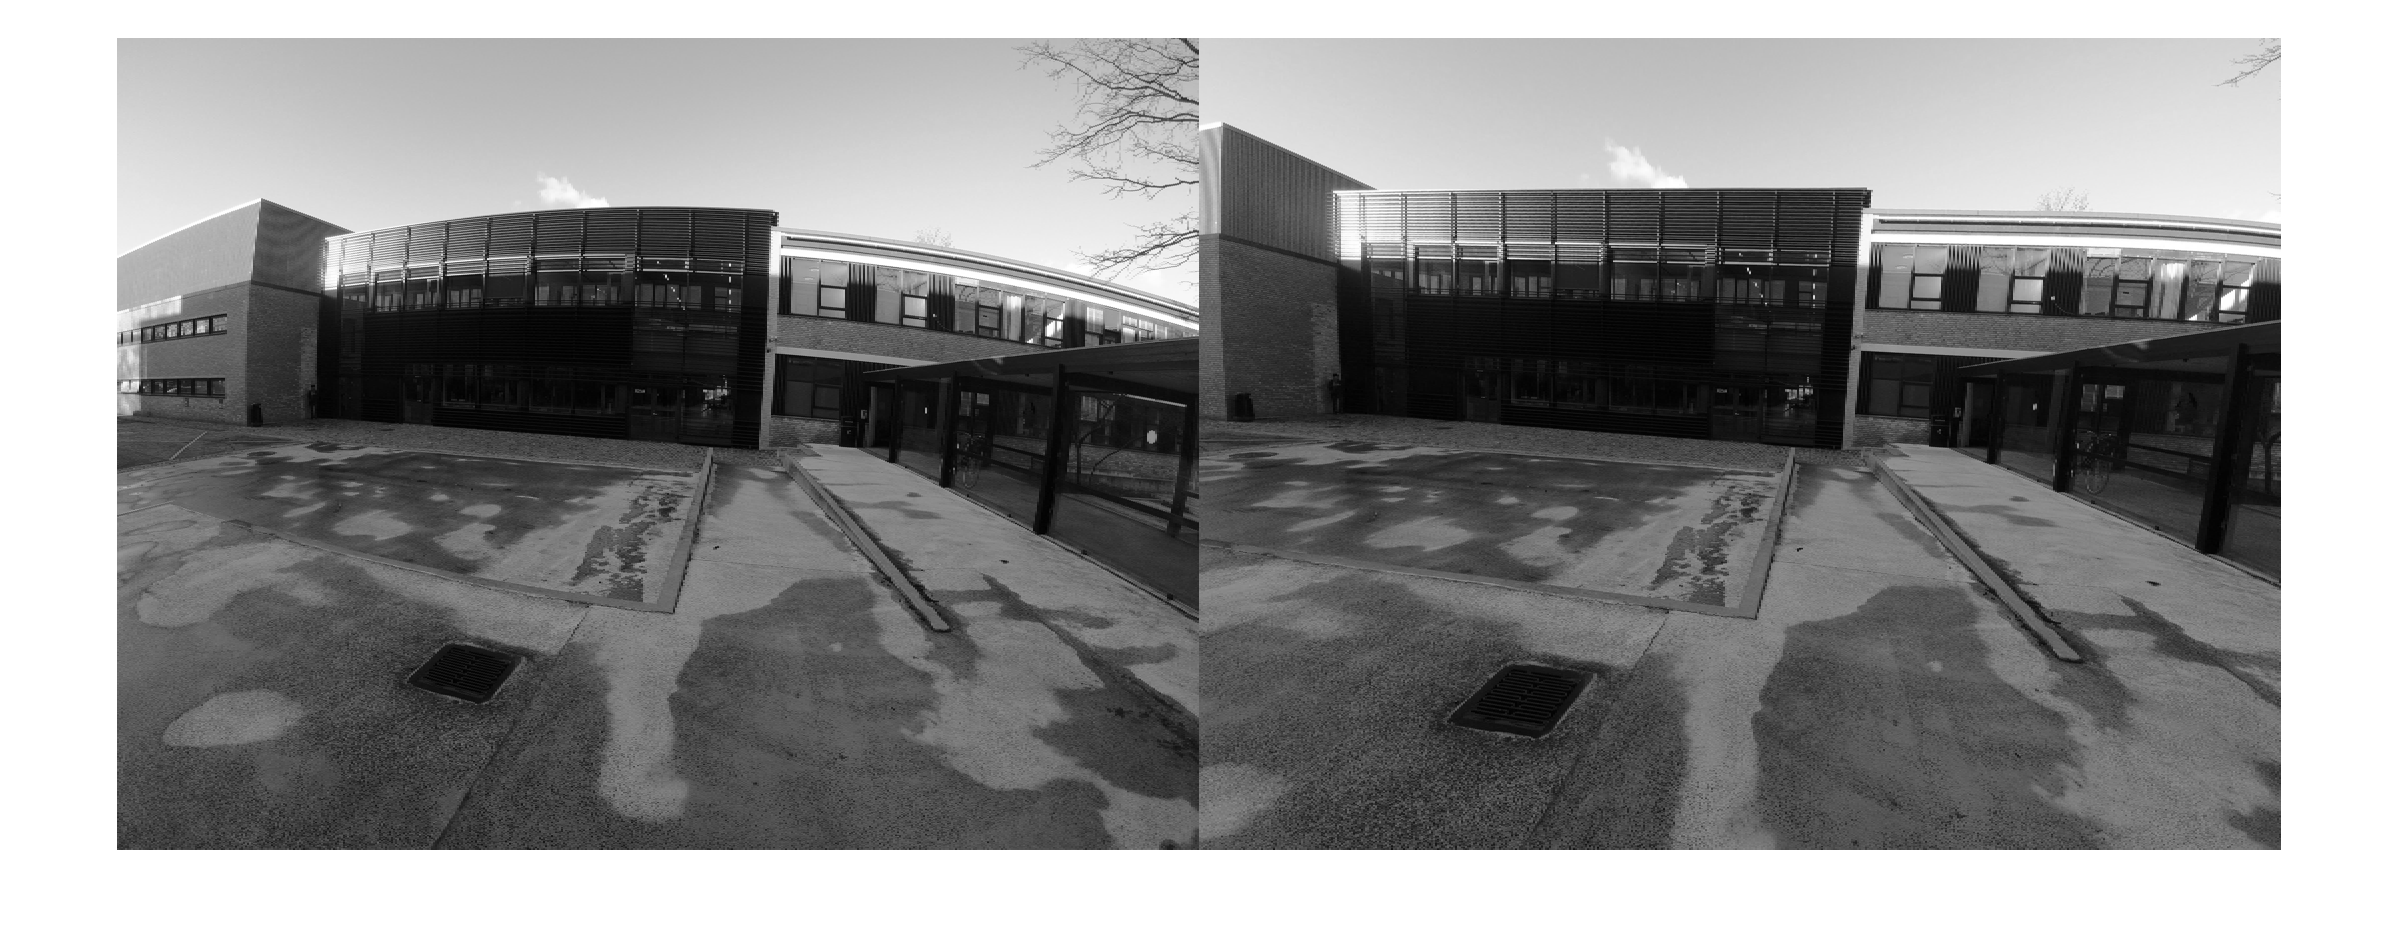
\includegraphics[scale=0.2]{figures/rec.png}
\caption{Example of undistorted and corresponding rectified image.}
\end{figure*}
\begin{enumerate}
\item read relevant docs to learn how to use those toolboxes.
\item load images prepared in the sub-folder \textbf{calibration} and complete camera calibration, use \textcolor{blue}{$112\ mm$} as the chessboard (or checkerboard) size.
\item verify the calibrated results and interpret the results you get.
\end{enumerate}
\paragraph{Q4:} 
Use the previous calibrated parameters to rectify a distorted image \textbf{distort.bmp}. 
\textbf{Hints:}
Recall that the distortion models are nonlinear, so it is not trivial to directly find the undistorted points from distorted points with known distorsion parameters. In stead, we can do it as follows:
\begin{itemize}
	\item Initialize a blank image.
	\item For each pixel $(x,y)$, compute the so called normalized coordiante $(x',y')$ as $x'=\frac{x-p_x}{f_x},\ y'=\frac{y-p_y}{f_y}$.
	\item Apply the radial and tangent distorsions to $(x',y')$ and denote the result as $(x_d,y_d)$ as
	\begin{align*}
		r^2 &= x'^2+y'^2 \\
		x'' &= x'(1+a_1r^2+a_2r^4+a_3r^6)+(2p_1x'y'+p_2(r^2+2x'^2)) \\
		y'' &= y'(1+a_1r^2+a_2r^4+a_3r^6)+(p_1(r^2+2y'^2)+2p_2x'y') \\
		x_d &= f_xx''+p_x\\
		y_d &=f_yy''+p_y
	\end{align*}

	\item Find the nearest neighbor of $(x_d,y_d)$ in distorted image and copy the corresponding intensity (or RGB) for $(x,y)$. 
\end{itemize}
Better results can be obtained by applying bilinear interpolation.


\section{Perspective $3$ Point}
Load the \textbf{p3p.mat} which contains:
\begin{itemize}
\item $\mathbf{K}$: simulated camera intrinsics;
\item $\mathbf{R}_i,\ \mathbf{t}_i,\ i=1,2,3$: ground truth extrinsics;
\item $\mathbf{x}_i,\ \mathbf{X}_i,\ i=1,2,3$: $\mathbf{X}_i$ denotes raw $3$D point and $\mathbf{x}_i$ represents the corresponding image point of $\mathbf{X}_i$, i.e. $$\mathbf{x}_i \sim \mathbf{K}(\mathbf{R}_i\mathbf{X}_i+\mathbf{t}_i)$$
\end{itemize}
The Perspective $3$ Point can be decoupled into $2$ steps
\begin{enumerate}
\item Recover the $3$D points in camera coordinate system (recall the lectures on cosine rule, fourth order polynomial, etc).
\item Use provided code \textbf{lssol.m} to recover the extrinsics.
\end{enumerate}
You should use $3$ points for the Perspective $3$ Point algorithm. Since multiple solutions may be obtained, you need at least a fourth point to choose the correct one. If you have more then $4$ points, you can select the best one by computing the re-projection errors for all points and select the one with the minimum re-projection error:
\begin{align*}
\text{Apply extrinsics: }\mathbf{x}'_i&=\mathbf{K}(\mathbf{RX}_i+\mathbf{t}),\\
\text{Homogeneous to inhomogeneous: } \mathbf{x}'_i&= \frac{\mathbf{x}'_i}{\mathbf{x}'_i(3)}  \\
\text{Compute reprojection error: }\mathbf{R^*}, \mathbf{t^*}&=\underset{\mathbf{R}, \mathbf{t}}{argmin}\ \sum_{i=1}^{n}||\mathbf{x}'_i-\mathbf{x}_i||\\
\end{align*}

You can check your recovered results using the following code:
\lstinputlisting{p3p.m}
Result obtained:
\begin{figure*}[!b]
\centering
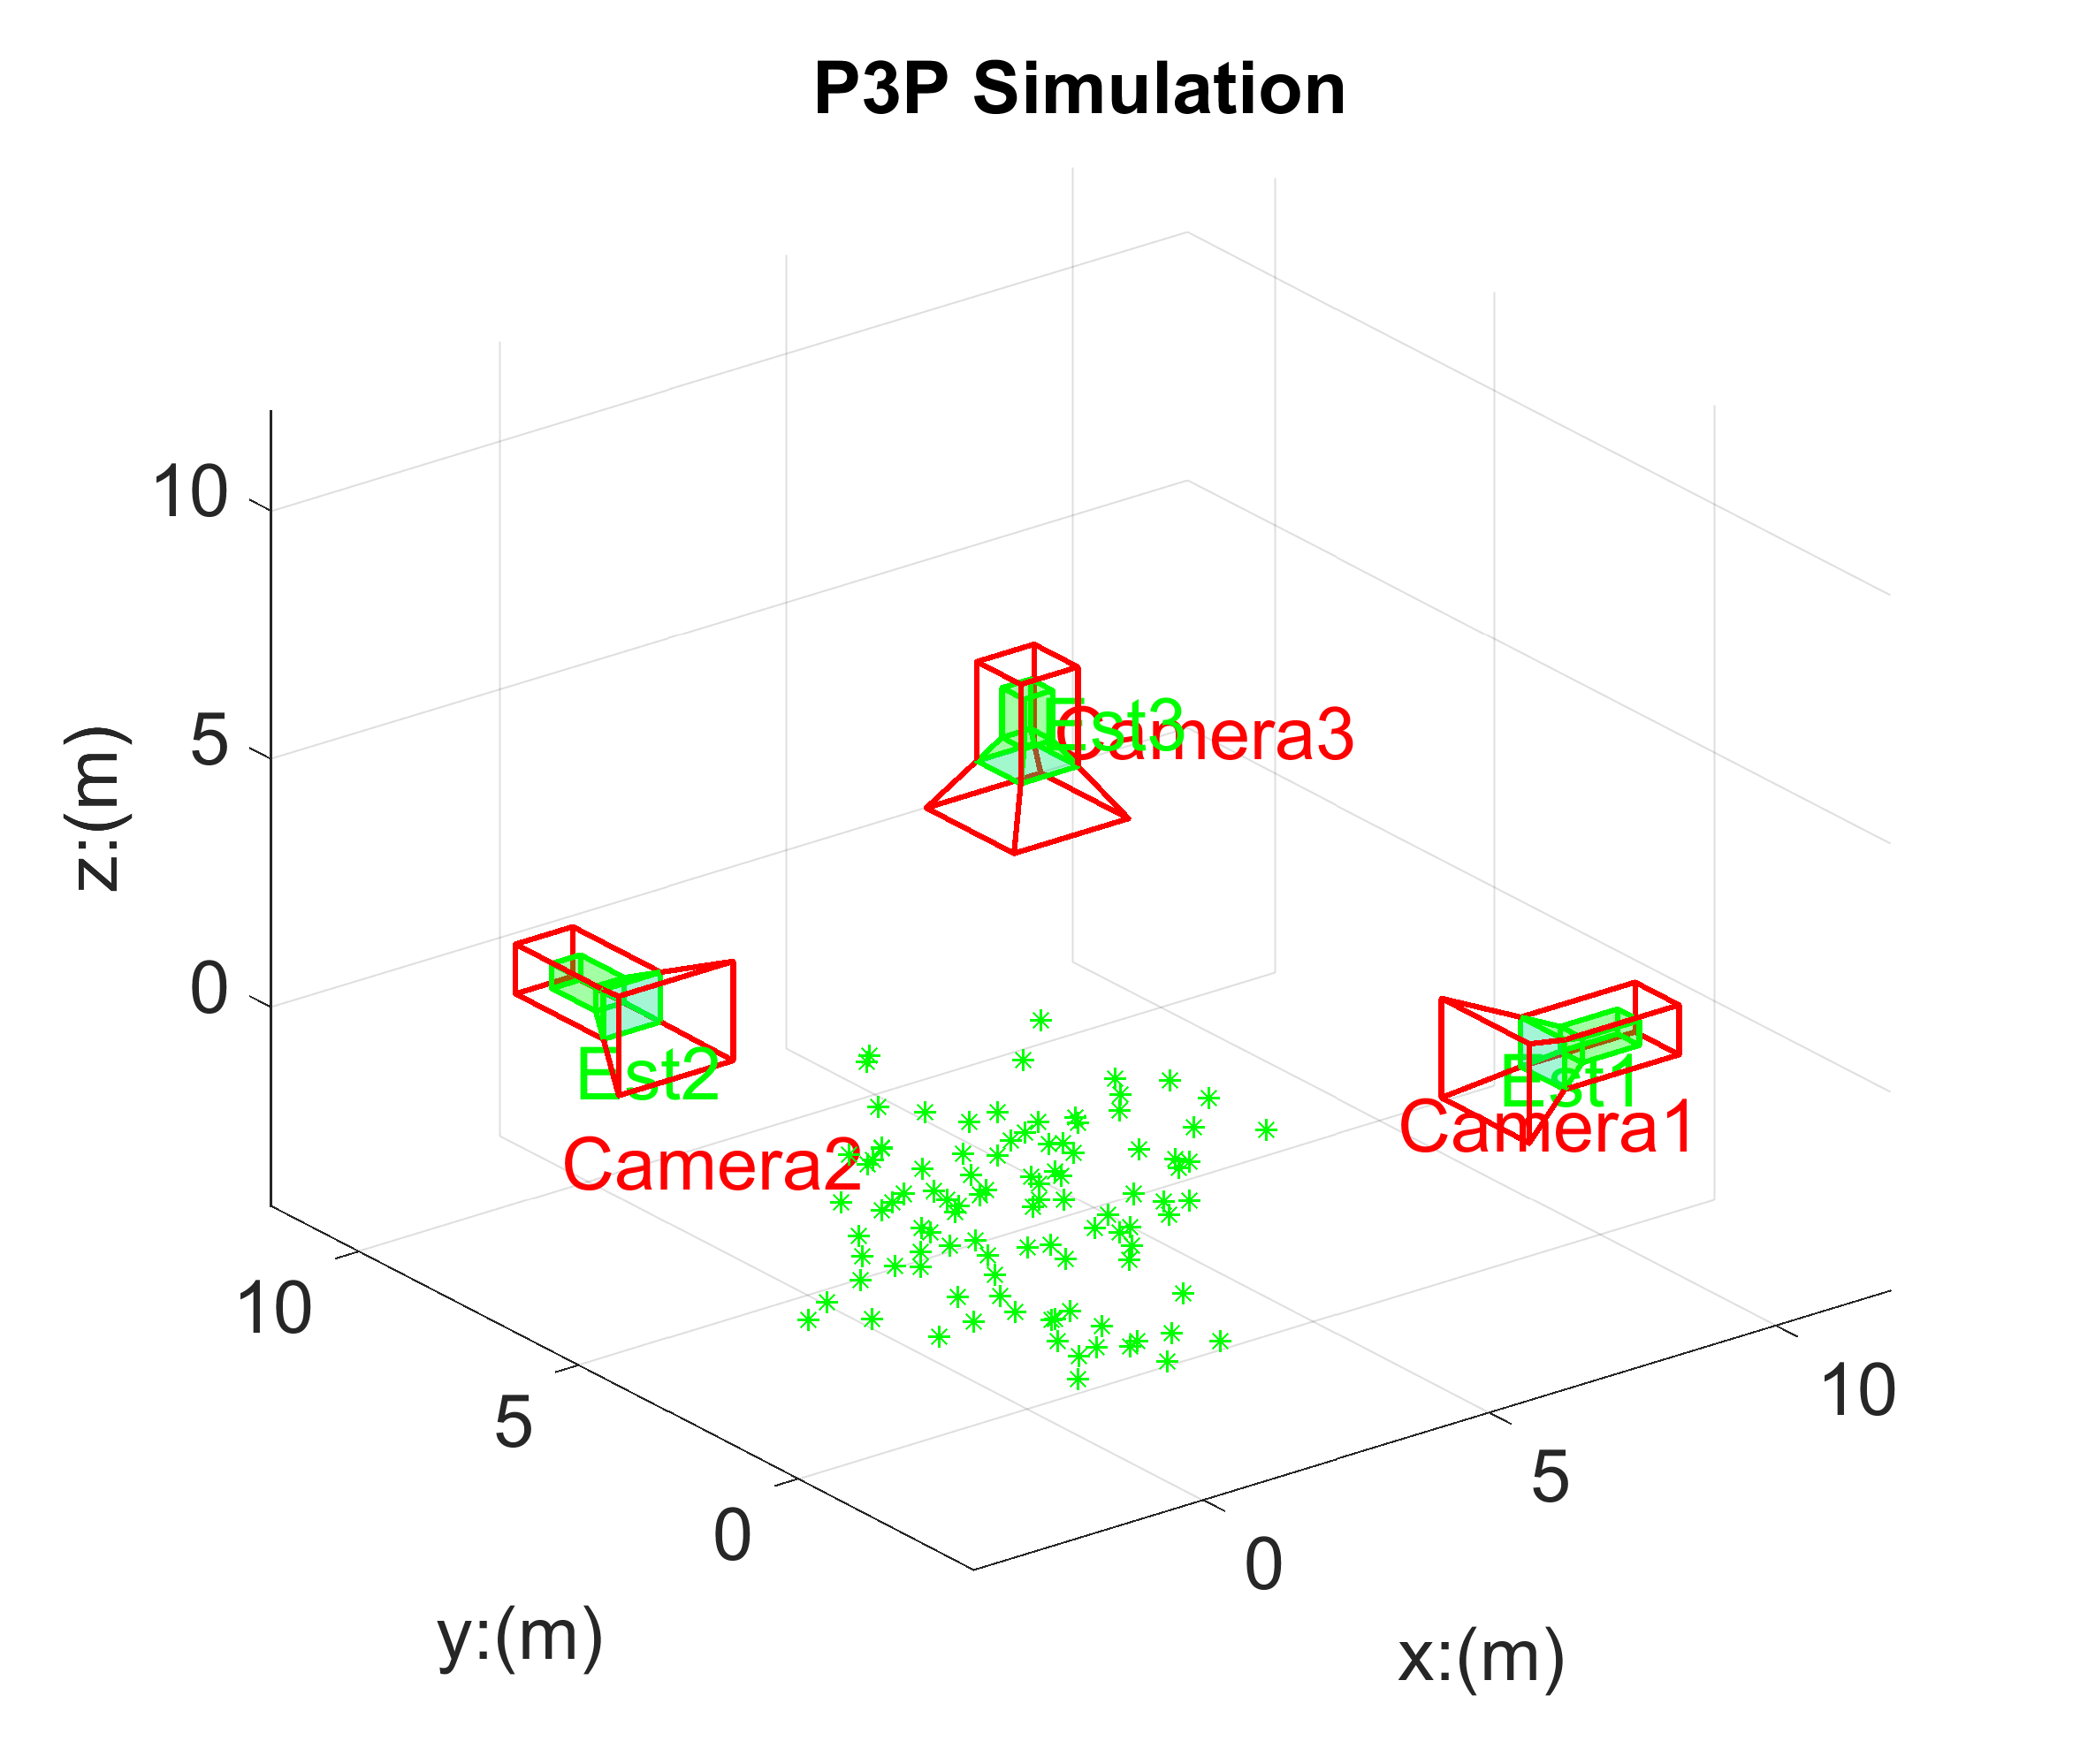
\includegraphics[scale=0.9]{figures/p3p.png}
\caption{Result obtained by applying Perspective-$3$-Point Method.}
\end{figure*}


%
%\section{Inverse Perspective Mapping}
%\paragraph{Q9:} Here you will work on how to remove the perspective effect by using the vanishing line and 2D transformation. Use the following code to load and display the image you will work:
%\lstinputlisting{ipm1.m}
%Then click on the displayed image to obtain the coordinates of four points you clicked. \textbf{q} will contain their homogeneous coordinates. You should work from here.

%In this attachment, you will find two supplementary files.
%\begin{itemize}
%\item \textbf{drawlines.m} - draw lines on image I.
%\item \textbf{warpping.m} - warp image I by transformation matrix $\mathbf{H}$. So after you find $\mathbf{H}$, call this function to get the resultant image.
%\end{itemize}
%%If you succeed, you will have a similar image like
%\begin{figure*}[!b]
%\centering
%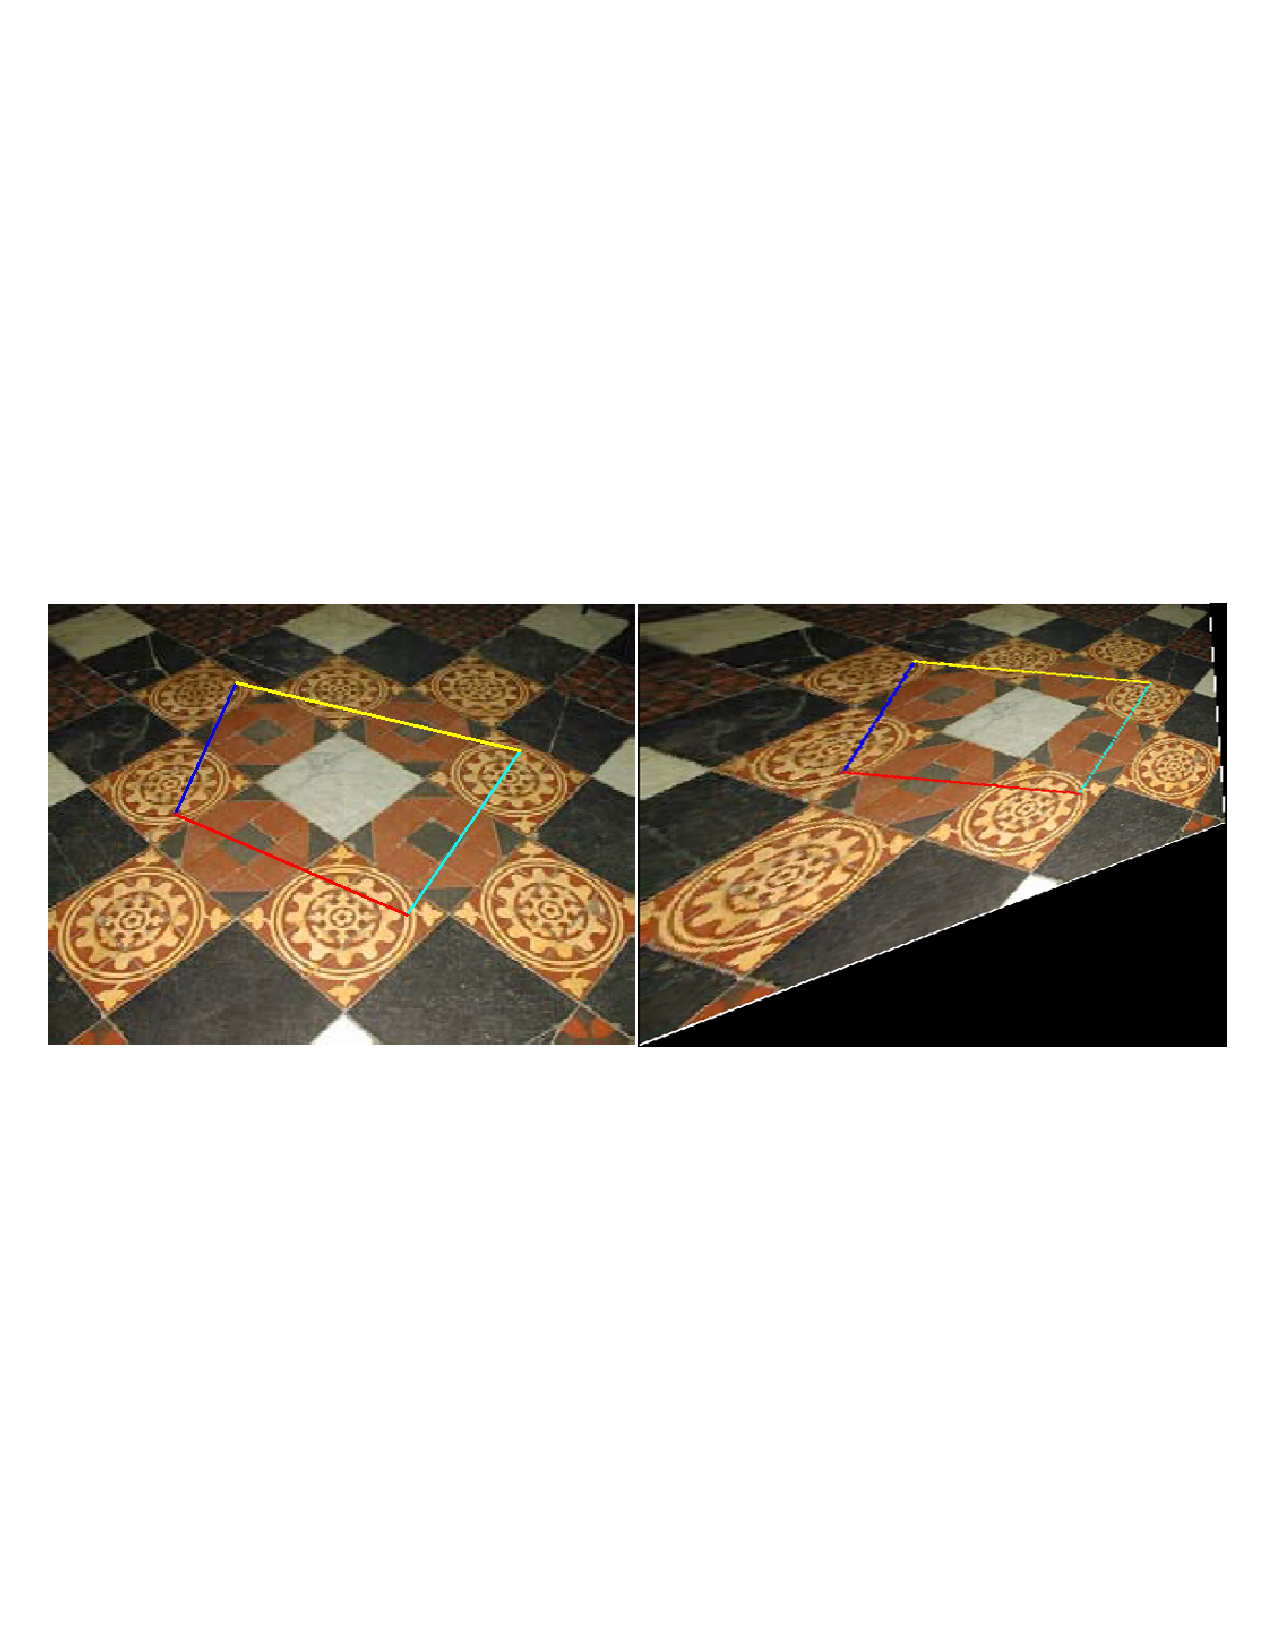
\includegraphics[scale=0.6]{figures/ipm}
%\caption{Illustration of the inverse perspective mapping.}
%\end{figure*}


 
\bibliography{hand_eye_calibration} 
\bibliographystyle{ieeetr}

\end{document}